\section{Genetsko programiranje}
\emph{Genetsko programiranje} (\emph{GP}) je evolucijski algoritam koji do rješenja dolazi iterativno mjenjajući populaciju sve dok uvjet zaustavljanja nije zadovoljen \cite{conv_gen_programming}.

\subsection{Jedinka populacije}
Jedinka populacije u genetskom algoritmu predstavlja jedno moguće rješenje na problem koji smo postavili.
Svaka jedinka je definirana s dvije stavke:
\begin{itemize}
	\item{Genotip}
	\item{Načinom mapiranja genotipa u \emph{fenotip}}
\end{itemize}
Na najnižoj razini, svaka jedinka je jedan genotip. 
Najčešće, genotip je prikazan kao niz brojeva, simbola ili bitova (~\ref{fig:gen_alg_tree_1}) \cite{naturally_selecting_algorithms}.
Korisnik koji koristi \emph{genetski algoritam} (GA) za pronalazak rješenja mora također definirati mapiranje $genotip \rightarrow fenotip$.
Genotipom možemo smatrati ono što koristi algoritam kako bi stvorio fenotip.
Što to znači?
Ukoliko je zadatak GA iz skupa točaka provesti simboličku regresiju $A\sin(Bx + C)$ gdje su $A$, $B$ i $C$ nepoznate varijable genotip bi se mogao prikazati kao vektor s tri elementa tipa broj s pomičnim zarezom.
Dalje, pravilo mapiranja genotipa u fenotip bi moglo biti da element na prvom mjestu odgovara vrijednosti koju pridajemo varijabli $A$ i tako dalje za varijable $B$ i $C$ (~\ref{fig:genotype_phenotype_map}).

\begin{figure}
	\caption{Mogućnosti spremanja i korištenja genotipa tijekom izvođenja genetskog algoritma}
	\begin{subfigure}[t]{0.45\textwidth}
		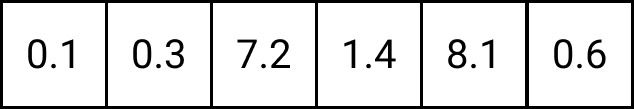
\includegraphics[width=\textwidth]{Illustrations/float_genotype.png}
		\caption{Genotip prikazan brojem s pomičnim zarezom}
	\end{subfigure}
	\hspace{\fill}
	\begin{subfigure}[t]{0.45\textwidth}
		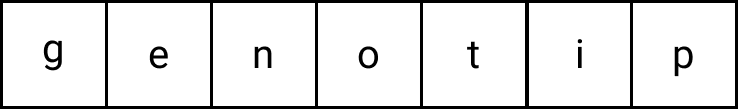
\includegraphics[width=\textwidth]{Illustrations/char_genotype.png}
		\caption{Genotip prikazan ascii znakovima}
	\end{subfigure}
	\label{fig:genotype_types}
\end{figure}

\begin{figure}
	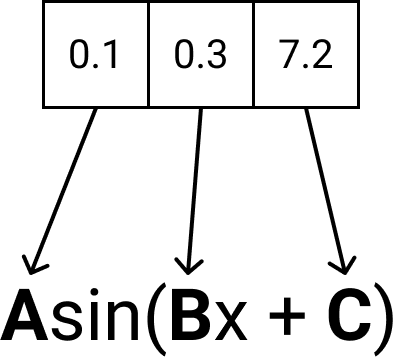
\includegraphics[width=0.4\linewidth]{Illustrations/genotype_phenotype_mapping.png}
	\caption{Primjer mapiranja genotipa u fenotip}
	\label{fig:genotype_phenotype_map}
\end{figure}
